\documentclass[11pt,a4paper]{article}
\usepackage{fontspec}
\setmainfont{TeX Gyre Pagella}
\newfontfamily\headfont{Inter}[UprightFont=*-ExtraBold,BoldFont=*-ExtraBold,Extension=.otf,Path=/usr/share/fonts/opentype/inter/]
\usepackage[a4paper,margin=2.3cm]{geometry}
\usepackage{graphicx,booktabs,float,caption,array,xcolor}
\usepackage[hidelinks]{hyperref}
\usepackage{titlesec}
\usepackage[round]{natbib}
\usepackage{setspace}
\setstretch{1.05}
\renewcommand{\topfraction}{0.9}
\renewcommand{\bottomfraction}{0.8}
\renewcommand{\textfraction}{0.1}
\renewcommand{\floatpagefraction}{0.75}
\setlength{\parindent}{0pt}
\setlength{\parskip}{0.55em}
\titleformat{\section}{\headfont\Large}{\thesection}{0.8em}{}
\titleformat{\subsection}{\headfont\large}{\thesubsection}{0.8em}{}
\captionsetup{font=small,labelfont=bf}
\urlstyle{same}
\hypersetup{pdftitle={Roads of the Roman Empire: Certainty, Density, Straight Runs and Days from Rome in the Itiner-e Network},pdfauthor={Tristan Hotham}}

\begin{document}
\begin{center}
{\Large\bfseries Roads of the Roman Empire\par}
\vspace{0.4em}
{\large Certainty, density, straight runs and days from Rome\\in the Itiner-e network\par}
\vspace{1.2em}
{\large Tristan Hotham\par}
\vspace{0.3em}
{\small Independent researcher\\
ORCID: 0000-0003-4931-9349\\
DOI: \detokenize{10.5281/zenodo.23857866}\par}
\vspace{0.8em}
2026
\end{center}

\begin{quote}
\small
\begin{center}\textbf{Abstract}\end{center}
Itiner-e is the most detailed open dataset yet of the roads of the Roman Empire: 14,769 road sections with a combined length of 299,171 km, each graded by how certain its course is. I describe the network and use it for a simple, fully stated travel-time model. Only 8,181 km (2.7\%) is graded certain; 90\% is conjectured and 7.4\% hypothetical. A fifth of the length (19\%) carries a date or the name of a builder. Treating the network as a graph of 10,315 junctions, with speeds from the middle of the ranges given in Wikipedia's article on Roman roads (22.5 km a day on foot, 45 by horse-drawn cart, 80 by courier), a slope penalty taken from the dataset's own passability field, and one day for each of four short sea crossings, London is 81 days on foot from Rome, Constantinople 75 and Alexandria, which by road must be reached round the eastern Mediterranean, 180. Carthage, 590 km from Rome, is 210 days by road, through Spain and across North Africa: a reminder that the empire's long journeys went by sea. The longest stretch of road that stays within 200 m of a straight line runs 56.1 km between Saint-Quentin and Amiens. Road density, measured in the provinces of about AD 117, is highest in Latium and Campania (144 km per 1,000 km\textsuperscript{2}) and outside Italy in Cyprus, Judaea and Lycia et Pamphylia; it reflects the intensity of modern research as well as ancient road building.

\textbf{Keywords:} Roman roads; Itiner-e; transport networks; travel time; network analysis; historical GIS; Roman Empire
\end{quote}

\section{Introduction}
Roads were among the most visible works of the Roman state. They carried armies, officials, letters and trade, and they tied the provinces to Italy and to each other. For most of the twentieth century the network was known from printed atlases and regional studies, culminating in the Barrington Atlas of the Greek and Roman World \citep{talbert2000}. Digital versions followed, among them the Digital Atlas of the Roman Empire \citep{dare} and the road layers of the Ancient World Mapping Center, and Stanford's ORBIS model turned a simplified network of roads, rivers and sea routes into a model of the cost of travel \citep{orbis,scheidel2014}.

Itiner-e, released in 2025, is a step change in detail \citep{itinere,desoto2025}. It digitises the roads section by section from atlases, survey and excavation reports, gazetteers, milestones, maps and aerial and satellite images, records the sources of each section, and grades each by how sure we are of its course. This paper uses the static 2024 version to ask four descriptive questions. How much of the network is known with certainty, and how much is dated? How long would it have taken to travel from Rome to the rest of the empire along these roads, under simple and stated assumptions? Where does the network run straightest? And where was it densest? An interactive version (\url{https://maps.tristanhotham.com/roman-roads/}) shows every section, the travel times from Rome or any other start, and the analyses below.

\section{Data}
The Itiner-e static version 2024 (Zenodo record version 1.3, \citealp{itinere}) holds 14,769 road sections in World Mercator. Each section runs between two places or road junctions and has a name built from its two end places, a type (main or secondary road), a certainty grade, start and end dates with error margins (rarely filled), the emperor or magistrate under whom it was built, the ancient itinerary or road name it belongs to, the person who digitised it and the bibliography, its geodesic length and its average slope. The field description defines the certainty grades: \emph{certain} sections are well documented and digitised to within 50 m in mountainous terrain and 200 m in the plains; \emph{conjectured} sections are identified roads whose course is less well documented; \emph{hypothetical} sections are roads that are identified but not localised, roads whose physical course was not fixed (in deserts and flood plains), or roads thought to have existed on insufficient evidence. The dataset also contains a passability value for every section, which the field description does not define (Section~\ref{sec:travel}).

Province outlines of about AD 117, with Italy divided into its eleven Augustan regions, and ancient place names used to label junctions come from the Digital Atlas of the Roman Empire \citep{dare}, through the open repository of its vector map. Land and modern place names are from Natural Earth \citep{naturalearth}. Travel speeds are taken from the English Wikipedia article on Roman roads \citep{wikiroads}, which states that horse-drawn carts could travel 40 to 50 km a day, pedestrians 20 to 25 km, and that a relay of horses could carry a letter about 80 km in a day.

\begin{table}[tbp]\centering\small\caption{Sources and licences.}\label{tab:sources}
\begin{tabular}{>{\raggedright\arraybackslash}p{4.4cm}>{\raggedright\arraybackslash}p{7cm}>{\raggedright\arraybackslash}p{3cm}}\toprule Source & Used for & Licence\\\midrule
Itiner-e static version 2024 & Roads, certainty, dates, builders, itineraries, slope, passability & CC BY 4.0\\
Digital Atlas of the Roman Empire & Provinces of about AD 117; ancient place names & As published by DARE\\
Wikipedia, `Roman roads' & Travel speeds; the 400,000 km estimate & CC BY-SA 4.0\\
Natural Earth & Land, coastlines, modern place names & Public domain\\
\bottomrule\end{tabular}\end{table}

\section{Methods}
\subsection{The network}
Section ends that lie within 1 m of each other are treated as one junction. At this tolerance the dataset is topologically clean: it yields 10,315 junctions, and one connected network that covers the mainland from Morocco and Portugal to Mesopotamia and Egypt, with separate networks on islands. Junctions are named by the place name shared by the sections that meet there, else by the nearest DARE place within a few kilometres. Dates come from the construction period field (the first year given, with Augustus alone read as 27 BCE, Julius Caesar as 49 BCE and `Tetrarchy or later' as 293 CE) and otherwise from the lower date field; a value of 9999 means not given.

\subsection{Travel times}\label{sec:travel}
The time to traverse a section, in days, is its length divided by the travel speed and by its passability. Speeds are the middle of Wikipedia's ranges: 22.5 km a day on foot, 45 km by horse-drawn cart and 80 km by courier; I also report times at the low and high ends of the ranges. The passability field is 1 for every section with an average slope below about 3.4 degrees and below 1 above it, down to 0.2 on the steepest section. For the 3,845 sections below 1 it matches $\exp(-3.5\tan s)$, where $s$ is the average slope, with a median absolute difference of 0.001: Tobler's hiking function relative to walking on the flat \citep{tobler1993}. I take it as the dataset's own slope penalty and apply it to all three modes. It covers 27\% of the length.

The roads stop at the sea. Four short crossings join them where the network meets the coast on both sides of a strait: the Channel (Gesoriacum to Dubris), the Strait of Messina, the Strait of Otranto (Brundisium to Dyrrachium) and the Strait of Gibraltar (Baelo to Tingi). Each counts as one day, whatever the mode. The Bosporus and Hellespont ferries are already in Itiner-e as short sections, and the bridge over the Euripus to Euboea is added as road. Shortest paths from the junction at the Forum in Rome are found with Dijkstra's algorithm \citep{dijkstra1959}. The time to a point off the network is the time to the nearest point on a road, plus the straight-line distance from it at half the road speed, up to 50 km. There are no rests, seasons, rivers, sea routes, tolls or borders, and the model gives the same time in both directions.

\subsection{Straight runs}
Long roads are made of many sections, so I first join sections into continuous lines through junctions where the road continues within 20 degrees of straight, pairing the straightest continuations first \citep{thomson1999}. Hypothetical sections, and the 306 sections described in the data as straight-line conjectures, are excluded. Each line is projected into a local azimuthal equidistant projection and simplified with the Douglas-Peucker algorithm at a tolerance of 200 m \citep{douglas1973}, the stated accuracy of a certain section in the plains. Each segment of the simplified line is a stretch where the digitised road never strays more than 200 m from a straight line; its length is the straight run. A conjectured stretch digitised with fewer than one vertex every 2 km is straight only because it was drawn that way, so such stretches are left out unless at least 90\% of the stretch is graded certain (276 stretches of 15 km or more removed).

\subsection{Density}
Every section is sampled at intervals of about 1 km and each piece of road is assigned to the DARE province that contains its midpoint. Density is road length per 1,000 km\textsuperscript{2} of the province's land area, measured in a Lambert azimuthal equal-area projection.

\section{Results}
\subsection{The network and its certainty}
The network totals 299,171 km, 7.5 times the circumference of the Earth. Main roads make up 103,478 km (35\%) and secondary roads 195,693 km. The median section is 13.0 km long; the longest, Dedris-Cydamus Ghadames in the Libyan desert, is 493 km and hypothetical. For comparison, Wikipedia's article states that the network comprised more than 400,000 km of roads, of which over 80,500 km were paved; Itiner-e's mapped total is 75\% of that figure.

Only 8,181 km, 2.7\% of the length (and 7.0\% of the sections), is graded certain (Figure~\ref{fig:cert}). 268,710 km (90\%) is conjectured and 22,281 km (7.4\%) hypothetical. Even among main roads only 5.4\% is certain, while 11\% of secondary roads are hypothetical. The certain kilometres are concentrated in the east, where surveys have been intensive and arid conditions preserve the line: Arabia, Syria, Galatia and Cappadocia and Judaea have the most.

\begin{figure}[tbp]\centering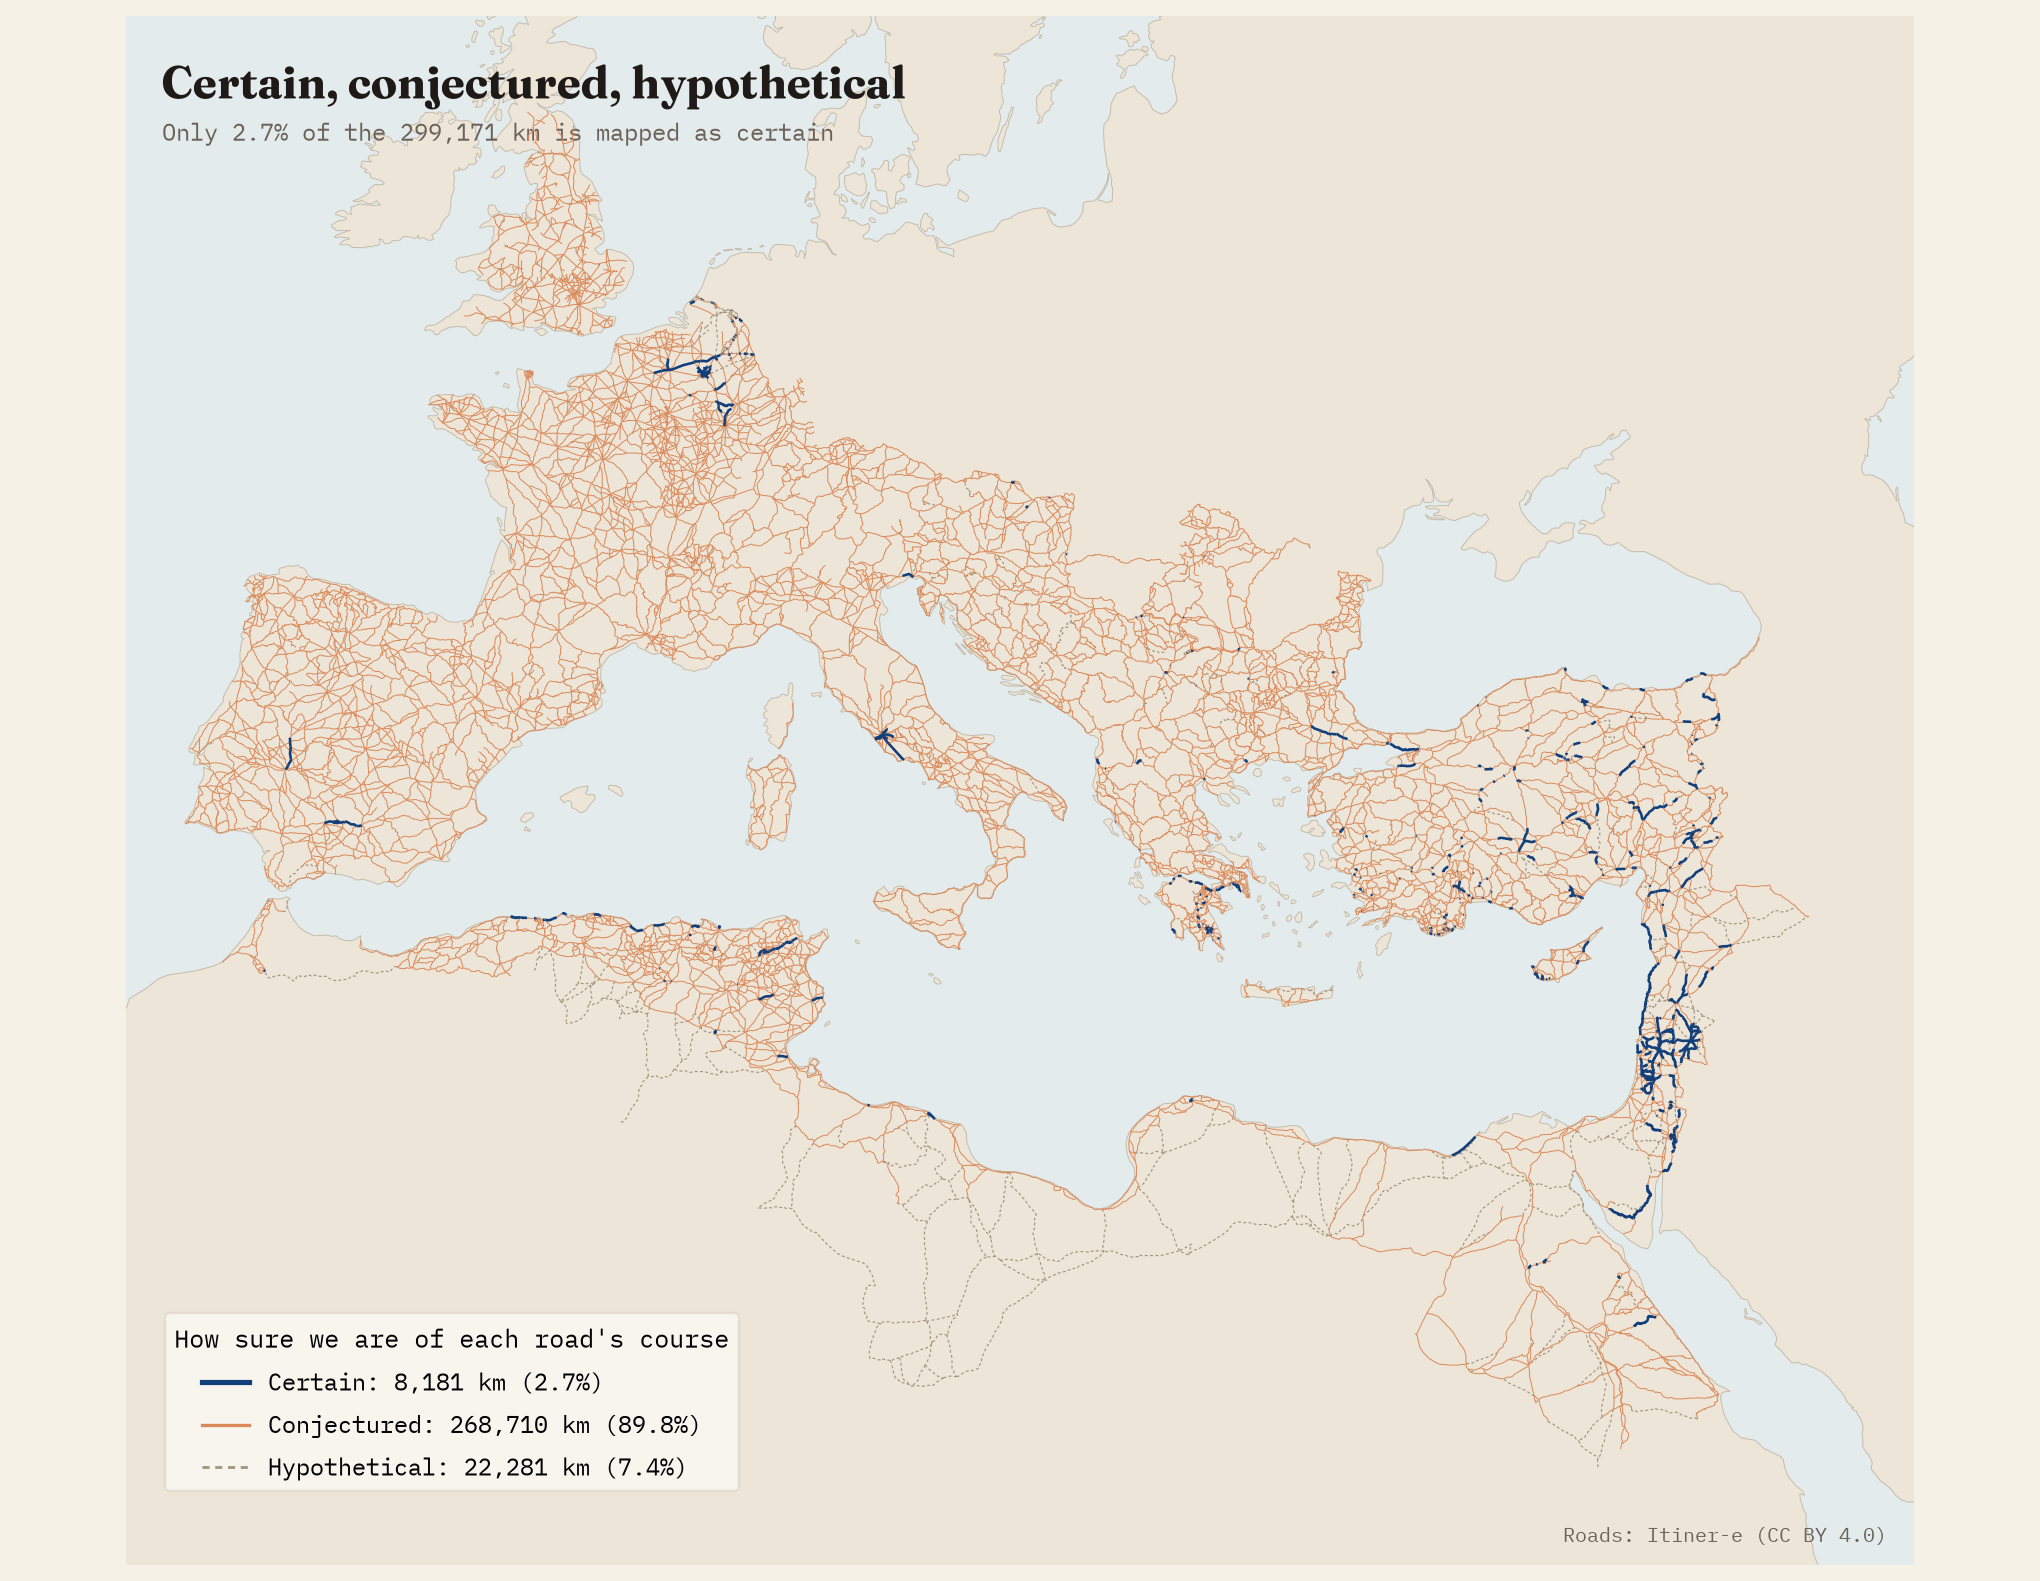
\includegraphics[width=\textwidth]{fig_certainty.png}\caption{The Itiner-e network by certainty of course. Certain sections are drawn thicker.}\label{fig:cert}\end{figure}

\subsection{Dates and builders}
3,176 sections (19\% of the length) have a date: 3,191 have a construction period and 477 a lower date; only 198 have an end date. Of the dated length, 7,469 km falls before 27 BCE, 10,845 km from 27 BCE to 68 CE, 15,637 km from 69 to 192 CE and 24,035 km in 193 CE or later. These counts follow the survival of milestones and inscriptions, and the attention of scholars, as much as the growth of the network. Claudius is named for the most kilometres (5,925 km), followed by Trajan (4,067 km) and Hadrian (3,932 km) (Figure~\ref{fig:builders}). 38\% of the length appears in at least one ancient itinerary: 75,486 km on the Tabula Peutingeriana and 68,861 km in the Antonine Itinerary. The longest named road in the data is the Via Egnatia (1,165 km).

\begin{figure}[tbp]\centering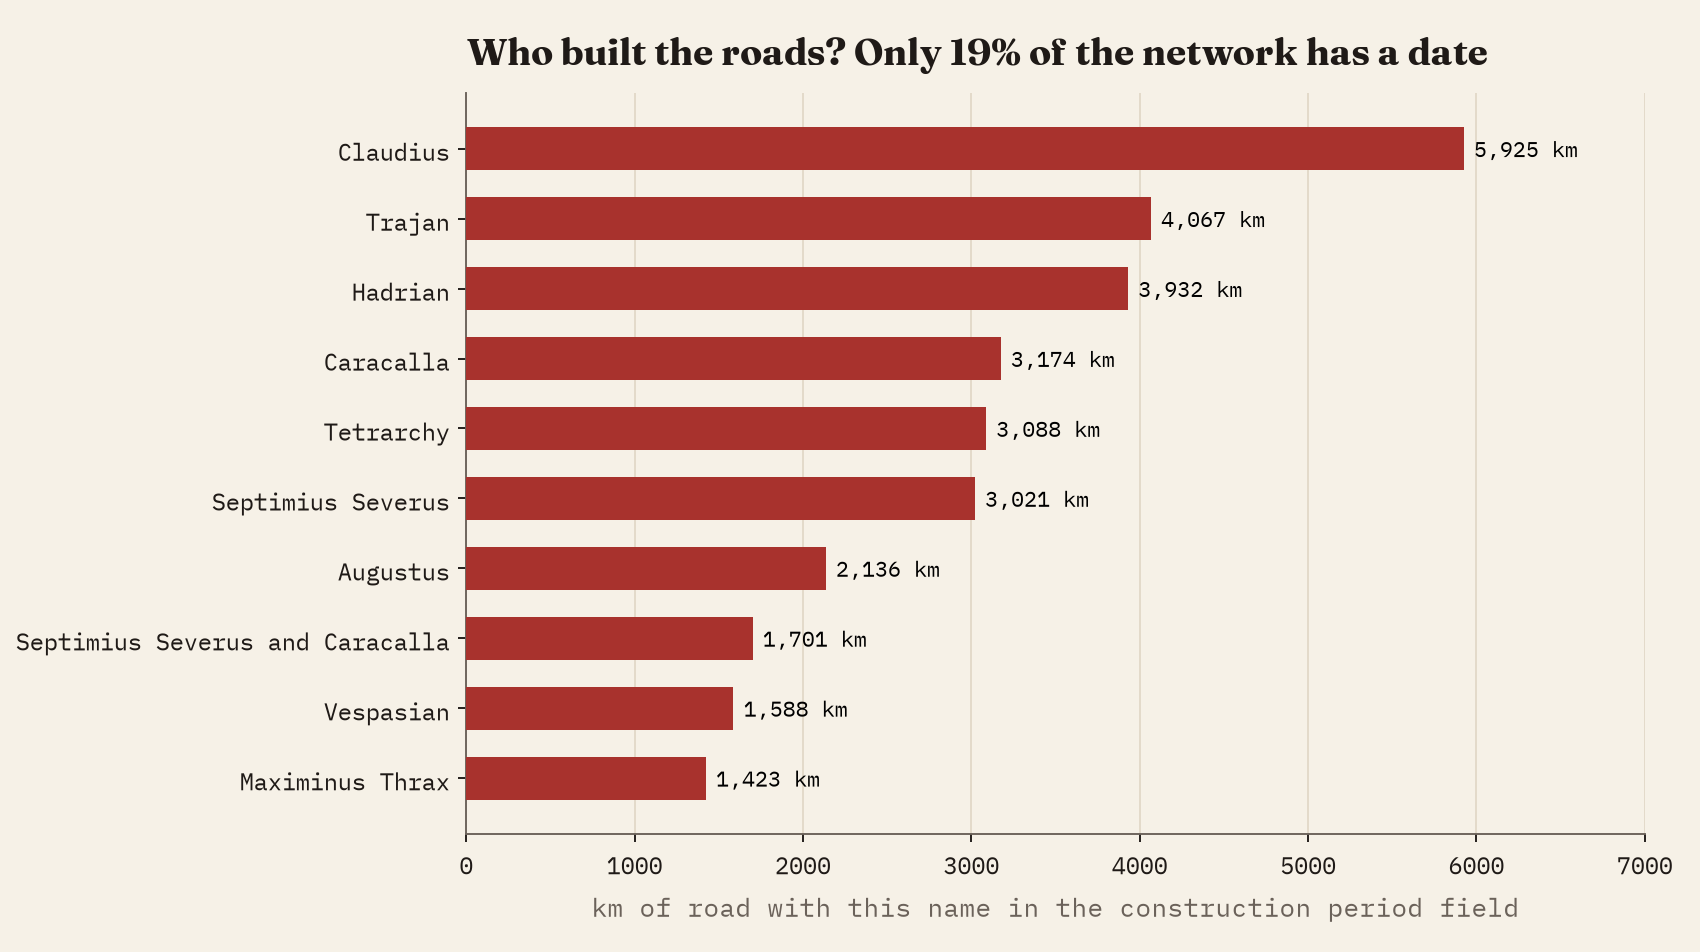
\includegraphics[width=.92\textwidth]{fig_builders.png}\caption{Road length by the emperor or magistrate named in the construction period field.}\label{fig:builders}\end{figure}

\subsection{Days from Rome}
Figure~\ref{fig:days} maps the modelled time on foot from Rome and Table~\ref{tab:cities} gives it for 20 cities. London is 81 days away on foot (73 to 91 days at 25 to 20 km a day), 41 by cart and 23 by courier, over 1,672 km of road and the Channel. Not one kilometre of that route is on a section graded certain. Constantinople is 75 days on foot by way of the Strait of Otranto and the Via Egnatia, and 107 days by land round the head of the Adriatic.

Alexandria is 180 days on foot: the road route crosses to Greece and runs through Asia Minor, Syria, Judaea and the Sinai, 3,807 km for a city 1,952 km from Rome. Carthage is further still, 210 days, by a route of 4,490 km through Gaul and Spain, across the Strait of Gibraltar and along North Africa, 7.6 times the straight-line distance. Only 5\% of the network lies within 30 days on foot of Rome, against 24\% by cart and 64\% by courier (Figure~\ref{fig:bands}). The furthest junction that can be reached is Murzuq in the Fezzan, 266 days on foot. 4,063 km (1.4\%) cannot be reached by road: the networks of Sardinia, Corsica, Crete and Cyprus and a few short fragments.

Two checks bound the role of the assumptions. Ignoring slope (passability set to 1) shortens the time to London to 75 days and to Alexandria to 169. Dropping every hypothetical section changes the times to Constantinople and Alexandria by less than a day (180.2 days to Alexandria against 179.9); in Britain, however, the final links into Londinium are hypothetical, so without them London cannot be reached.

\begin{figure}[tbp]\centering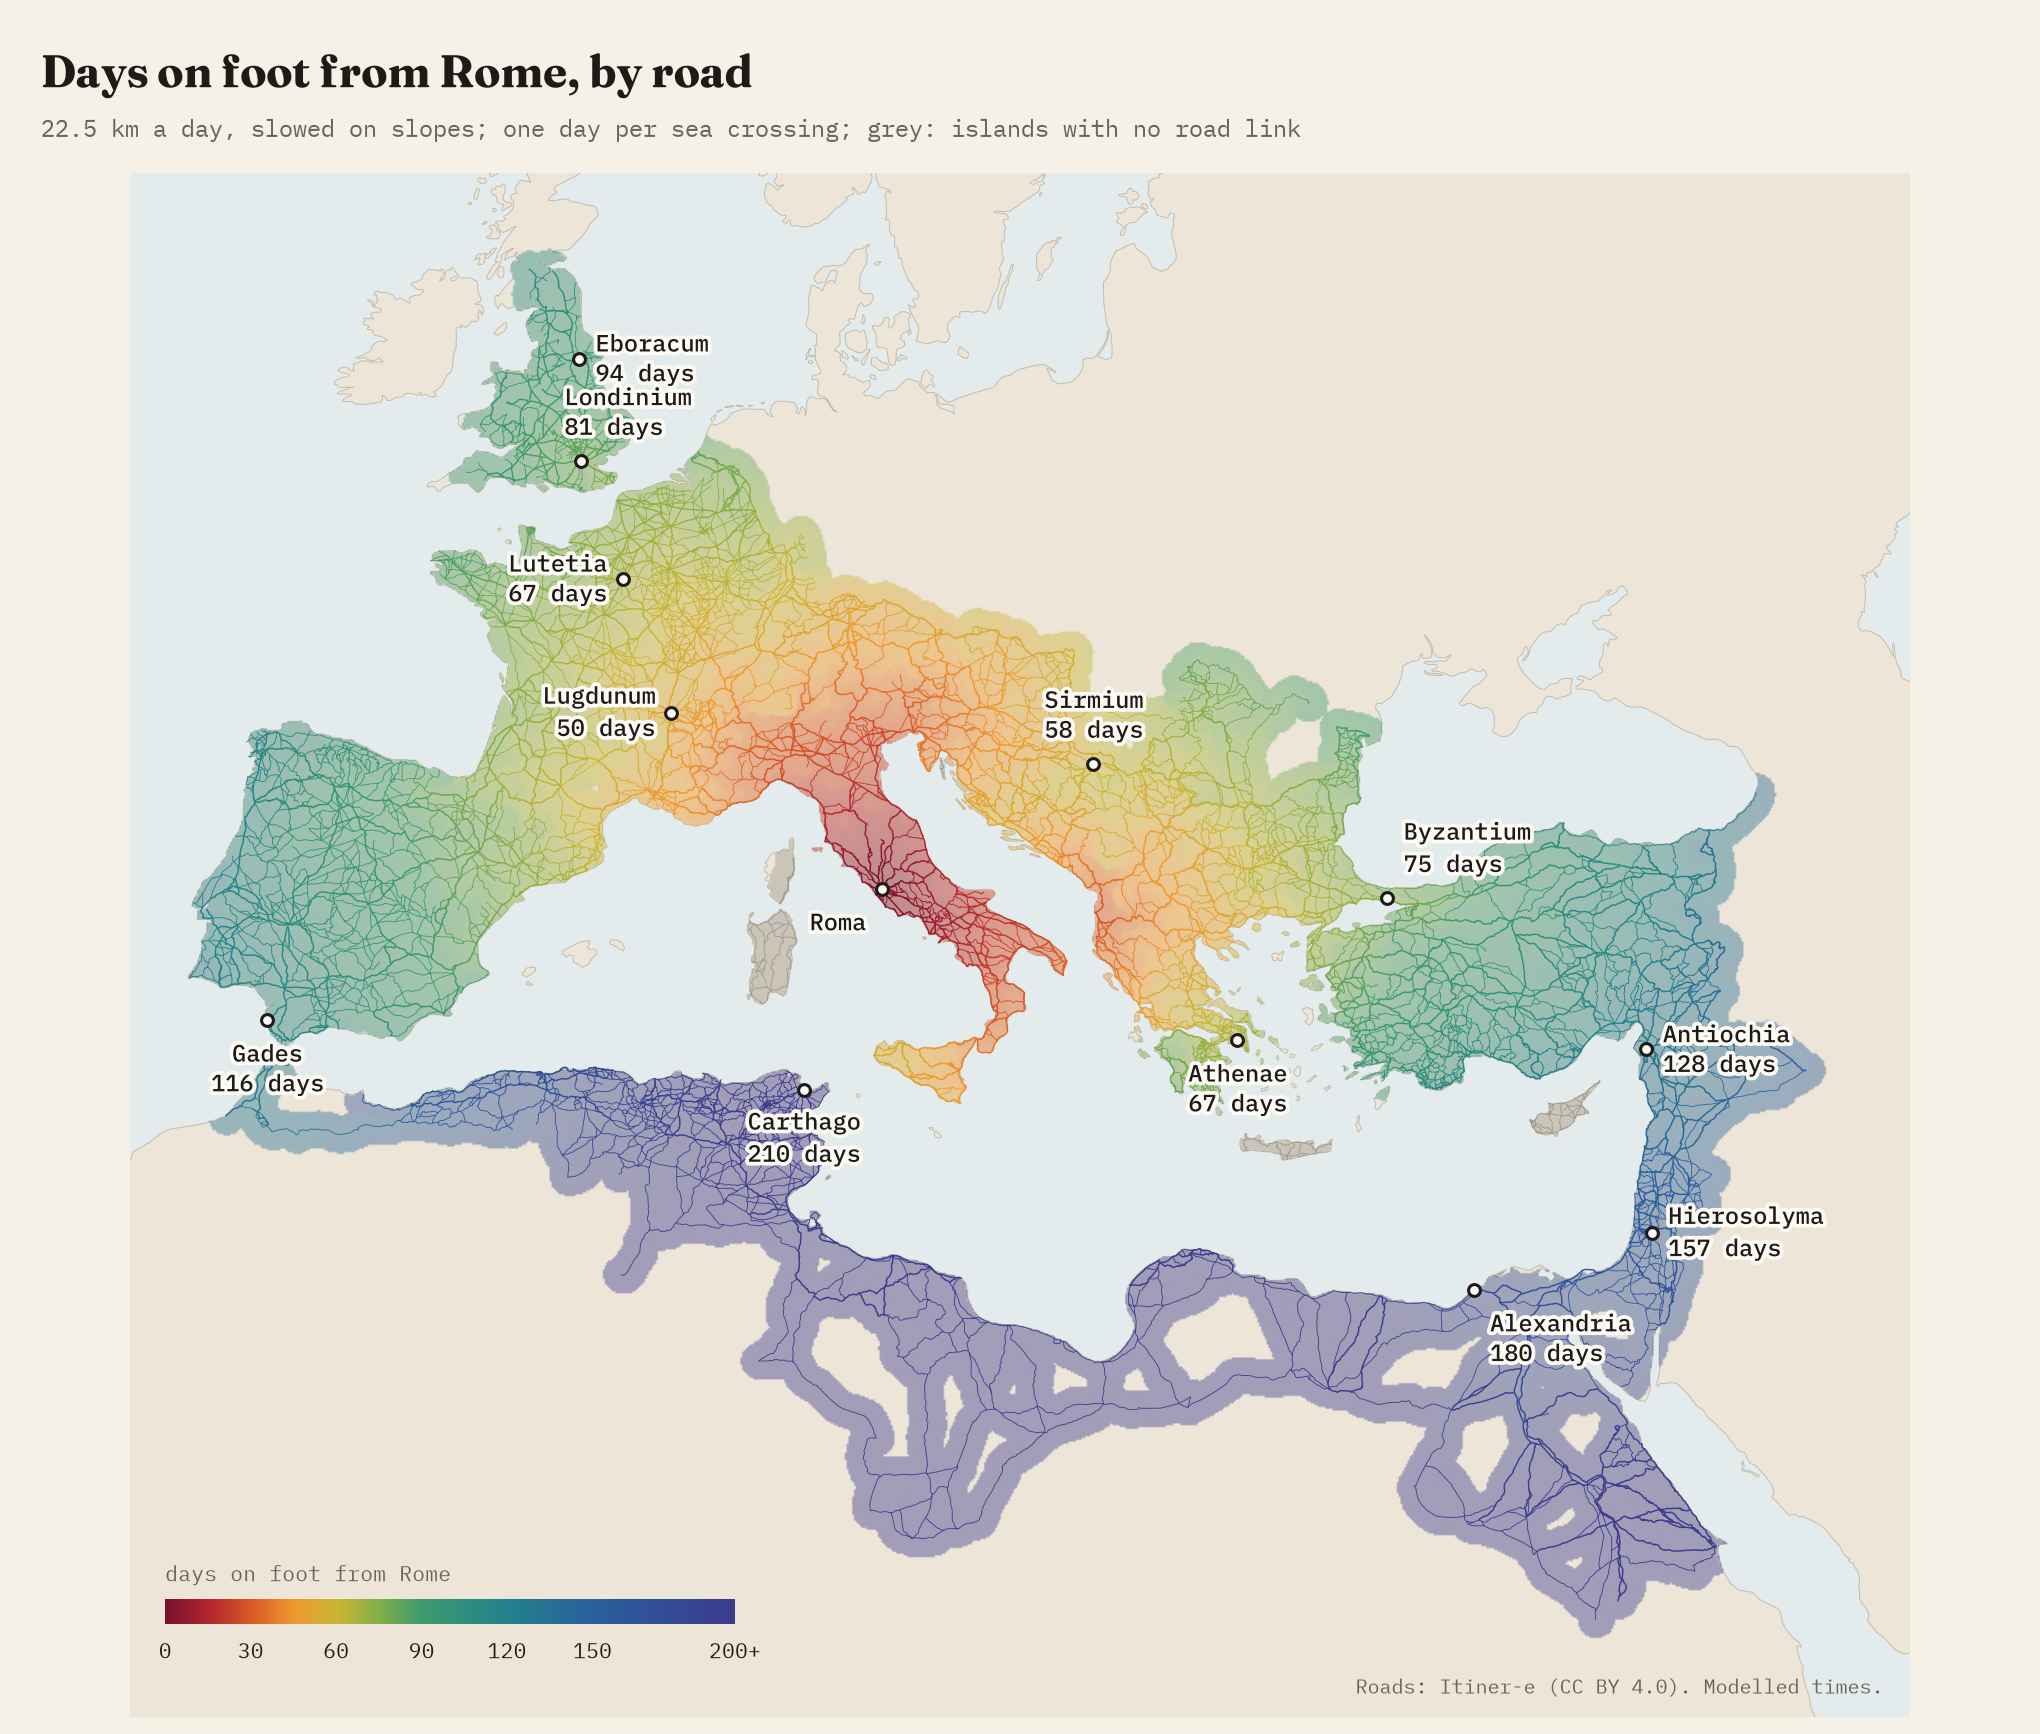
\includegraphics[width=\textwidth]{fig_days.png}\caption{Modelled days on foot from Rome. Roads are coloured by the time to the middle of each section; the shading shows the time to points up to 50 km off the road. Grey: islands with no road link to Rome.}\label{fig:days}\end{figure}

\begin{table}[tbp]\centering\small\caption{Modelled days from Rome. Road km: length of the quickest route on foot, excluding sea crossings. Range: on foot at 25 and 20 km a day.}\label{tab:cities}\begin{tabular}{llrrrrr}\toprule City & Ancient name & Road km & On foot & Range & Cart & Courier\\\midrule
Milan & Mediolanum & 607 & 28 & 26 to 32 & 14 & 8\\
Aquileia & Aquileia & 675 & 32 & 29 to 36 & 16 & 9\\
Lyon & Lugdunum & 990 & 50 & 45 to 56 & 25 & 14\\
Sremska Mitrovica & Sirmium & 1,243 & 58 & 52 to 65 & 29 & 16\\
Trier & Augusta Treverorum & 1,349 & 66 & 59 to 74 & 33 & 18\\
Paris & Lutetia & 1,387 & 67 & 60 to 75 & 33 & 19\\
Athens & Athenae & 1,352 & 67 & 60 to 75 & 34 & 20\\
Tarragona & Tarraco & 1,450 & 70 & 63 to 79 & 35 & 20\\
Cologne & Colonia Agrippina & 1,456 & 71 & 64 to 80 & 35 & 20\\
Constantinople (Istanbul) & Byzantium & 1,586 & 75 & 68 to 84 & 38 & 22\\
London & Londinium & 1,672 & 81 & 73 to 91 & 41 & 23\\
Ephesus & Ephesus & 1,864 & 88 & 80 to 99 & 45 & 26\\
York & Eboracum & 1,979 & 94 & 85 to 106 & 48 & 27\\
Mérida & Emerita Augusta & 2,231 & 108 & 97 to 121 & 54 & 30\\
Cádiz & Gades & 2,451 & 116 & 104 to 130 & 58 & 33\\
Antioch (Antakya) & Antiochia & 2,666 & 128 & 115 to 144 & 64 & 37\\
Jerusalem & Hierosolyma & 3,303 & 157 & 141 to 176 & 79 & 45\\
Alexandria & Alexandria & 3,807 & 180 & 162 to 202 & 90 & 51\\
Carthage & Carthago & 4,490 & 210 & 189 to 236 & 105 & 60\\
Leptis Magna & Lepcis Magna & 4,980 & 231 & 208 to 260 & 116 & 66\\
\bottomrule\end{tabular}\end{table}

\begin{figure}[tbp]\centering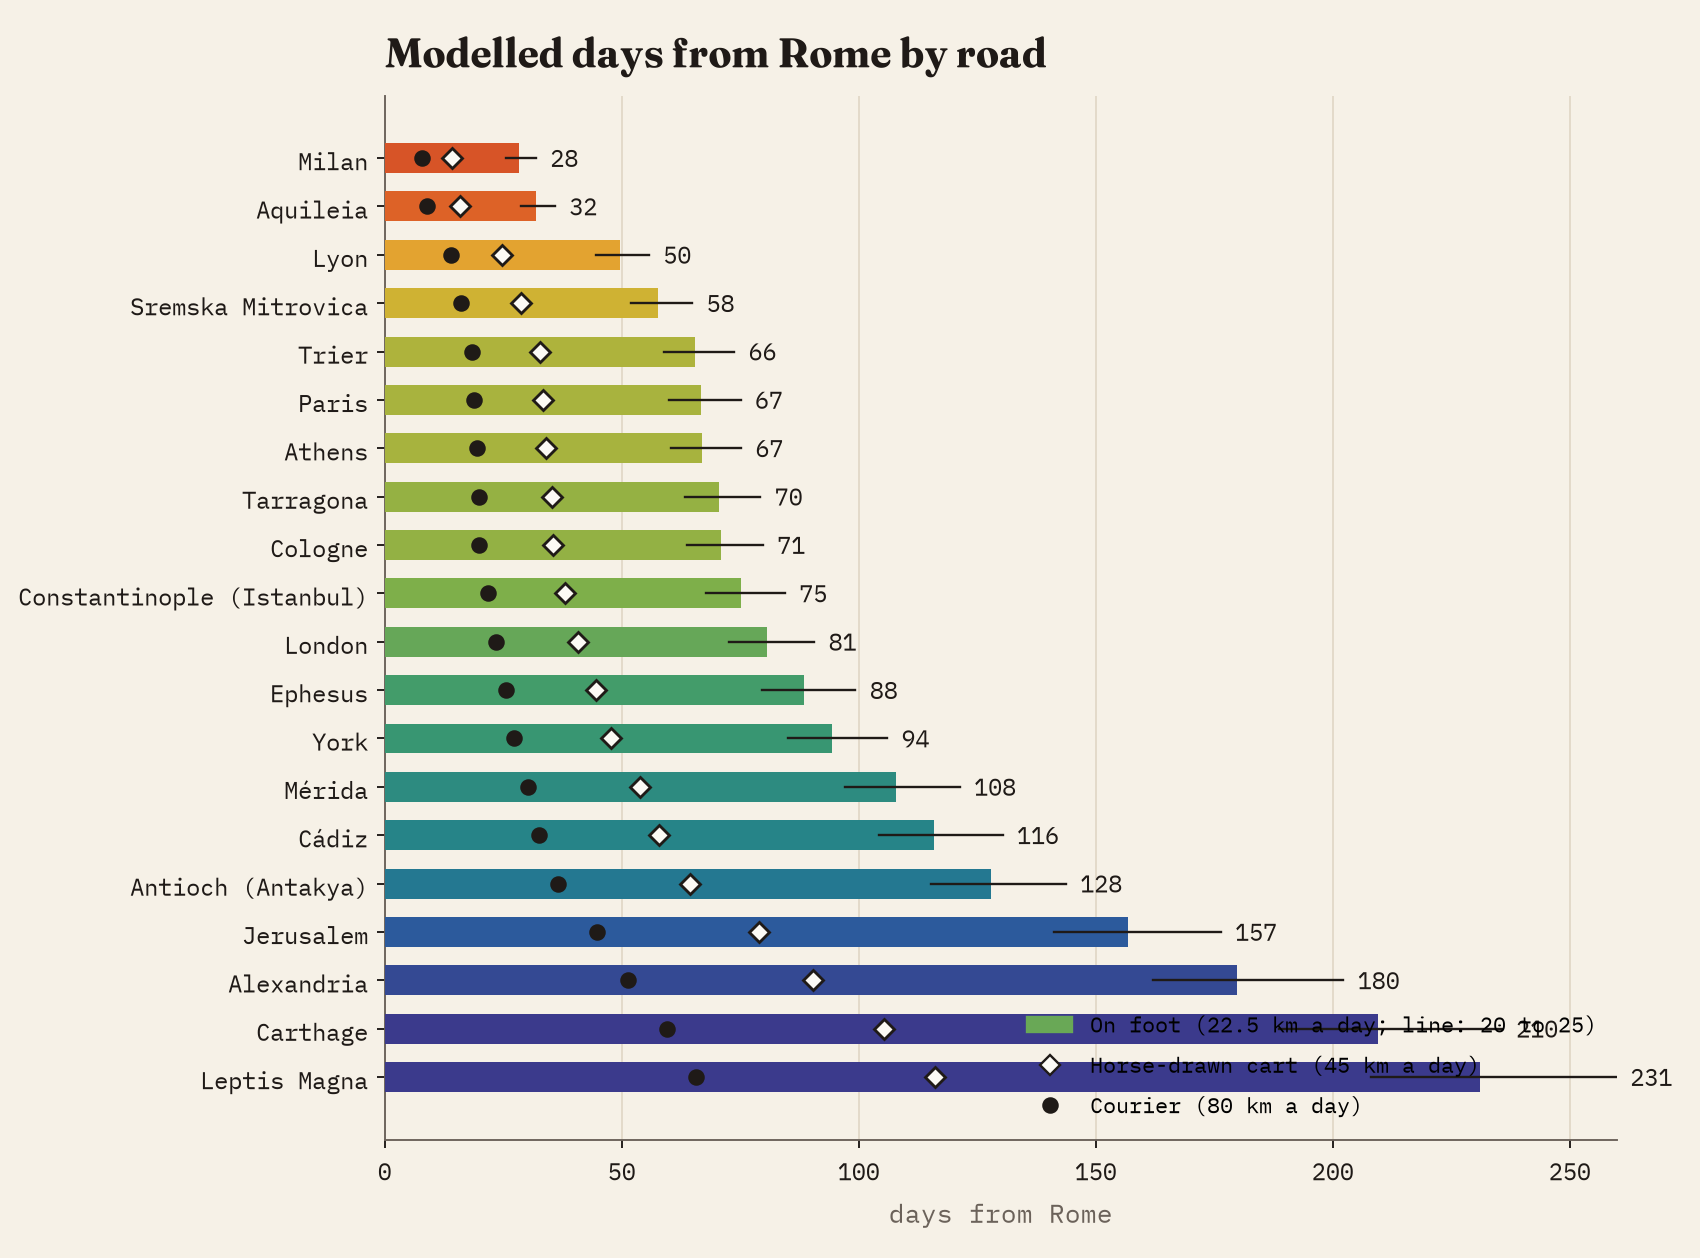
\includegraphics[width=.95\textwidth]{fig_cities.png}\caption{Modelled days from Rome on foot (bars, with the range for 20 to 25 km a day), by cart (diamonds) and by courier (dots).}\label{fig:cities}\end{figure}

\begin{figure}[tbp]\centering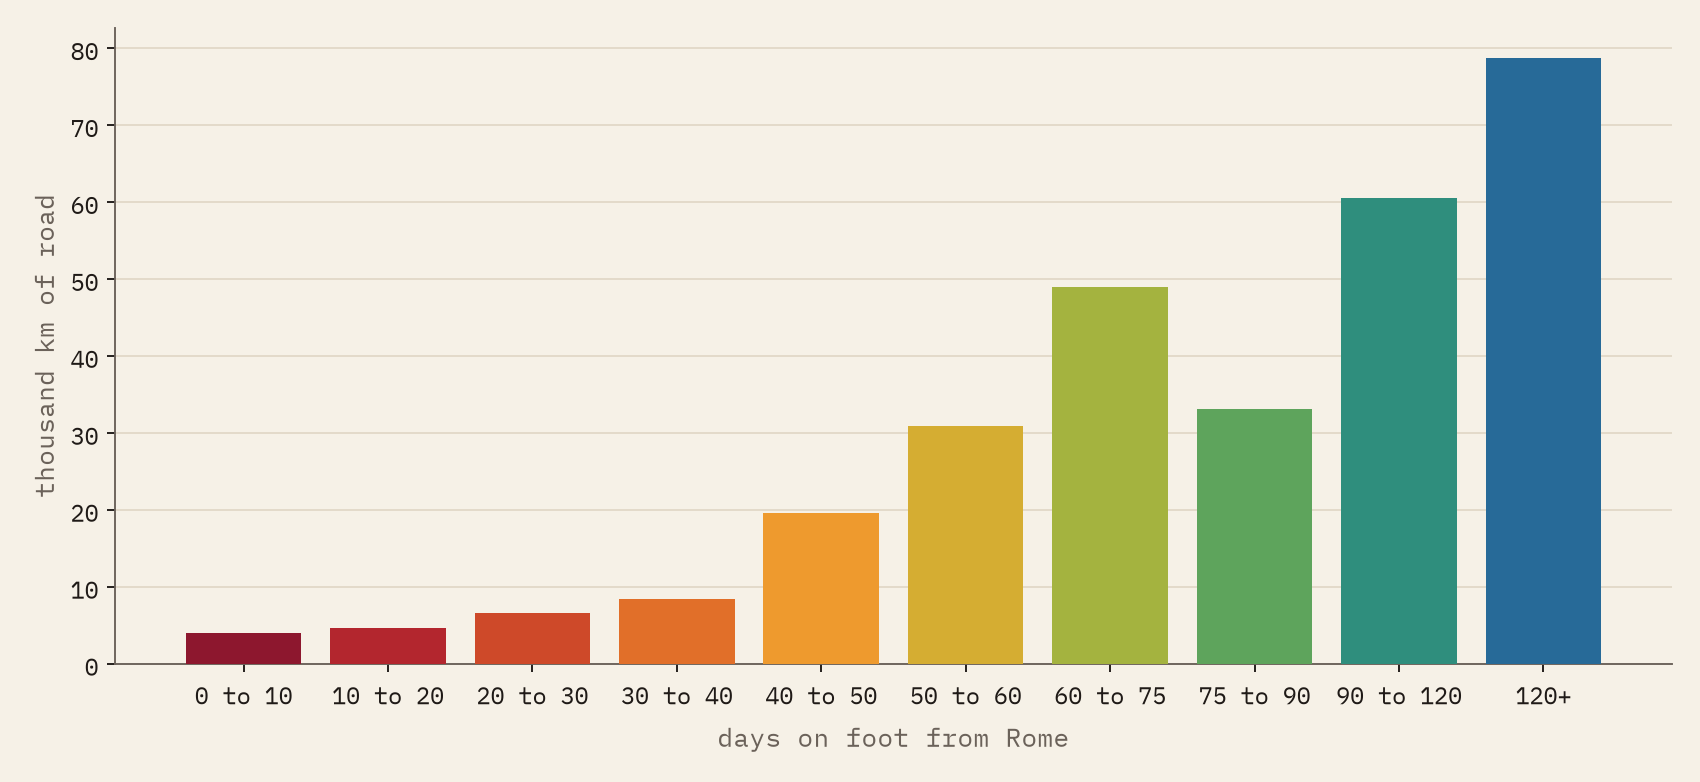
\includegraphics[width=.9\textwidth]{fig_bands.png}\caption{Road length by days on foot from Rome (time to the middle of each section).}\label{fig:bands}\end{figure}

\subsection{Straight runs}
46 stretches run straight to within 200 m for 20 km or more, and 7 for 30 km or more (Table~\ref{tab:runs}, Figure~\ref{fig:straight}). The longest, 56.1 km, lies between Saint-Quentin and Amiens in Picardy. It is followed by the Via Postumia between Vicenza and Concordia (49.4 km) and the Via Appia across the Pontine plain towards Terracina (42.0 km), which is the longest straight run on sections graded certain, with a largest deviation of 20 m. Several of the longest runs are in northern Gaul and on the Via Aemilia. The tolerance is strict: many well-known alignments bend slightly at river crossings or ridges and break into shorter runs.

\begin{table}[tbp]\centering\small\caption{The longest straight runs: stretches within 200 m of a straight line. Off line: largest deviation of the digitised road.}\label{tab:runs}\begin{tabular}{rp{8.2cm}rrr}\toprule & Stretch & km & Off line (m) & Certain\\\midrule
1 & Between Saint-Quentin and Amiens & 56.1 & 124 & 0\%\\
2 & Via Postumia, between Vicenza and Concordia & 49.4 & 109 & 0\%\\
3 & Via Appia, across the Pontine plain to Terracina & 42.0 & 20 & 100\%\\
4 & Via Belgica, between Heerlen and Cologne & 40.5 & 37 & 38\%\\
5 & Via Aemilia, east of Bologna & 33.7 & 59 & 0\%\\
6 & Nemetacum to Camaracum & 32.5 & 96 & 0\%\\
7 & Castrum Divionense to Andematunnum & 30.1 & 26 & 0\%\\
8 & Samarobriva to Saint Just en Chauseeée & 30.0 & 170 & 0\%\\
9 & Via Belgica, Bagacum to Furfooz & 28.4 & 128 & 100\%\\
10 & Via Aemilia, Veleia to Placentia & 27.8 & 171 & 0\%\\
\bottomrule\end{tabular}\end{table}

\begin{figure}[tbp]\centering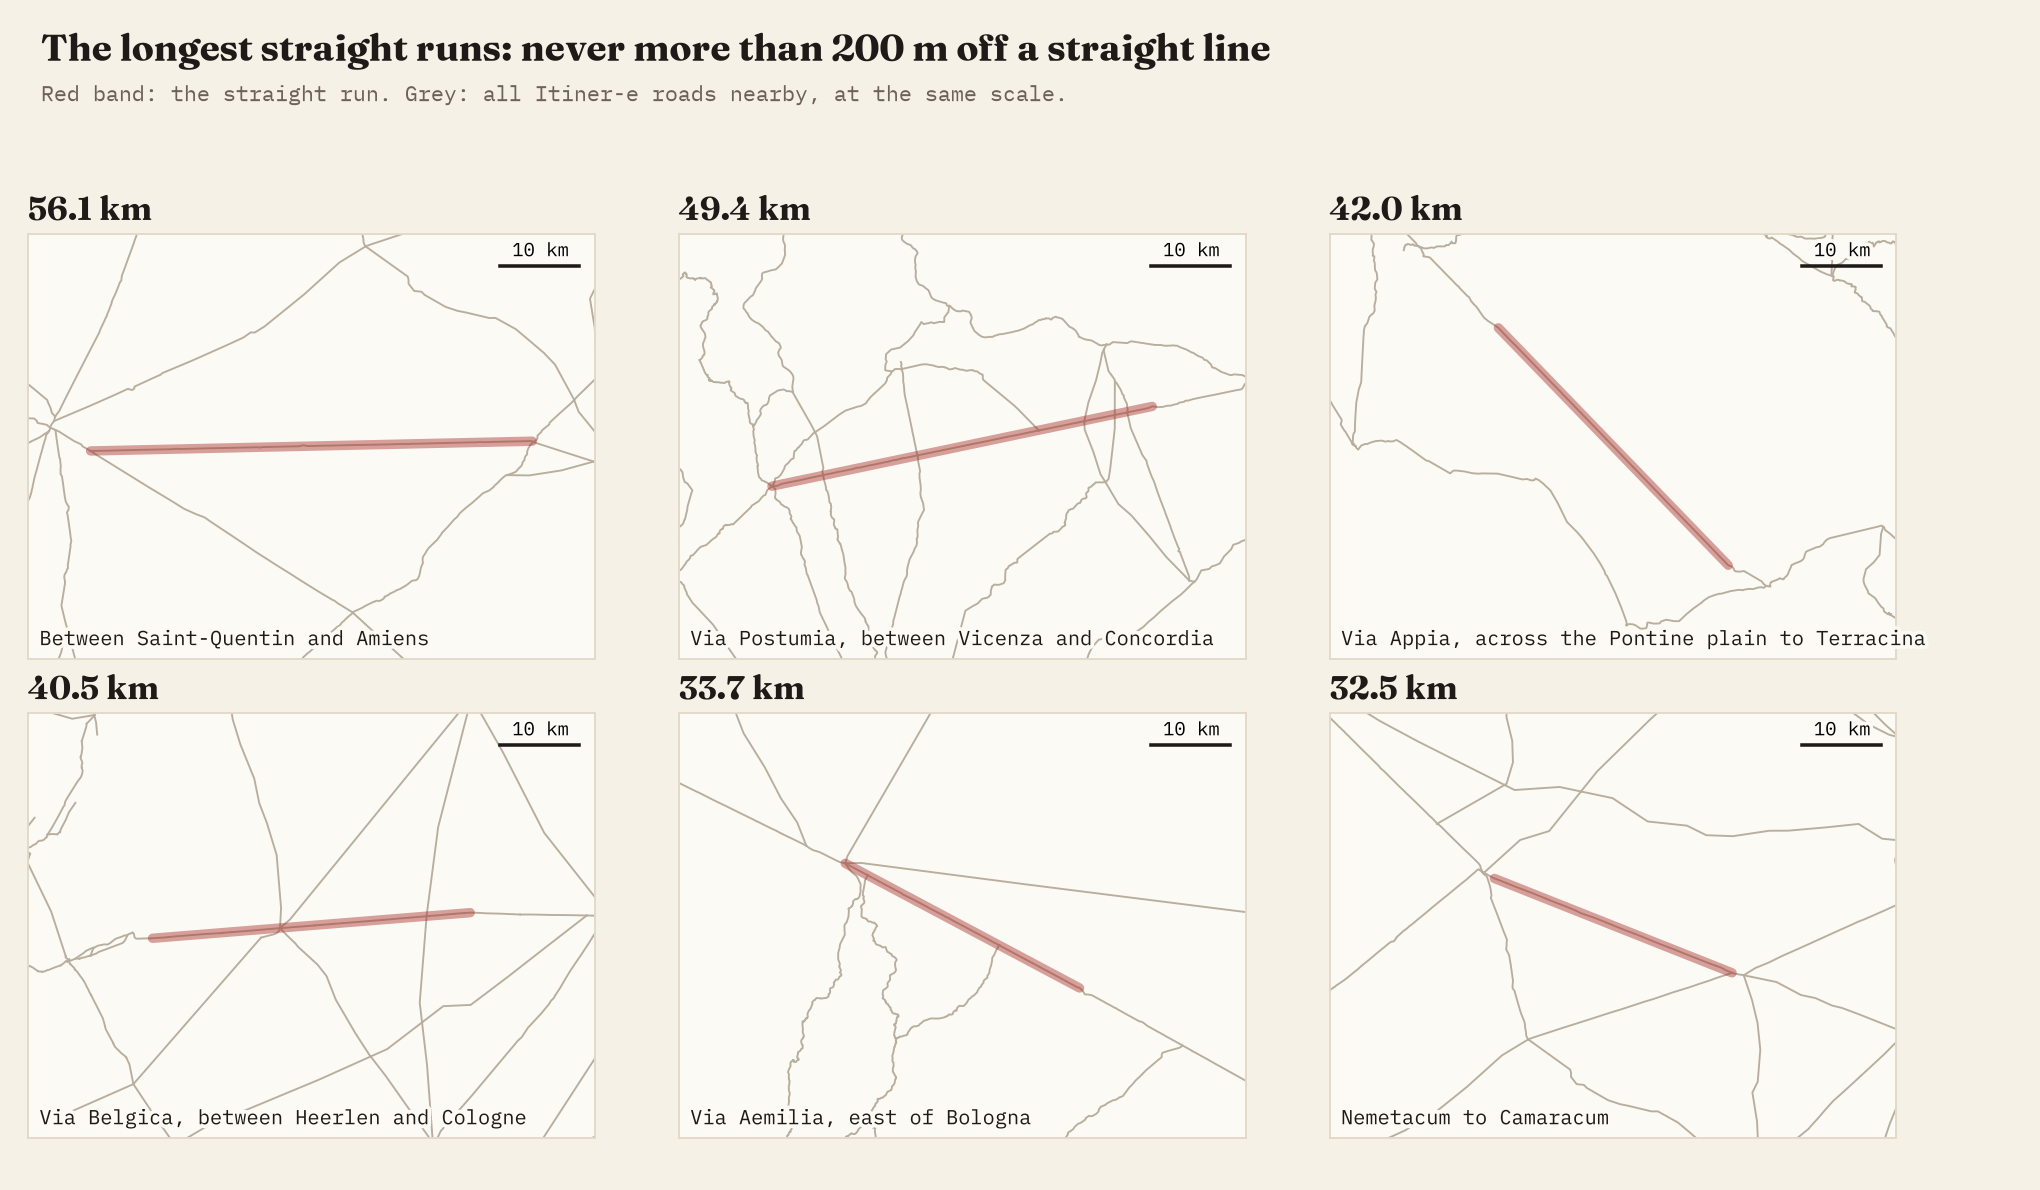
\includegraphics[width=\textwidth]{fig_straight.png}\caption{The six longest straight runs (red) with all Itiner-e roads nearby (grey), each at the same scale.}\label{fig:straight}\end{figure}

\subsection{Density by province}
Across the 53 provinces and regions, road density averages 58 km per 1,000 km\textsuperscript{2} (Figure~\ref{fig:prov}, Table~\ref{tab:prov}). It is highest in Italia, regio I (Latium et Campania) (144), and outside Italy in Cyprus (131), Judaea (130) and Lycia et Pamphylia (129). Italy as a whole has 70. The lowest densities are in provinces that were largely desert or held briefly: Egypt (24), Crete and Cyrene (20), Mauretania Tingitana (23) and Armenia and Mesopotamia (3.8). 15,732 km (5.3\%) lies outside the provinces. Density also tracks research: Judaea, with 39\% of its roads graded certain, is among the most intensively surveyed regions, while Umbria (regio VI, 31) is unexpectedly thin.

\begin{figure}[tbp]\centering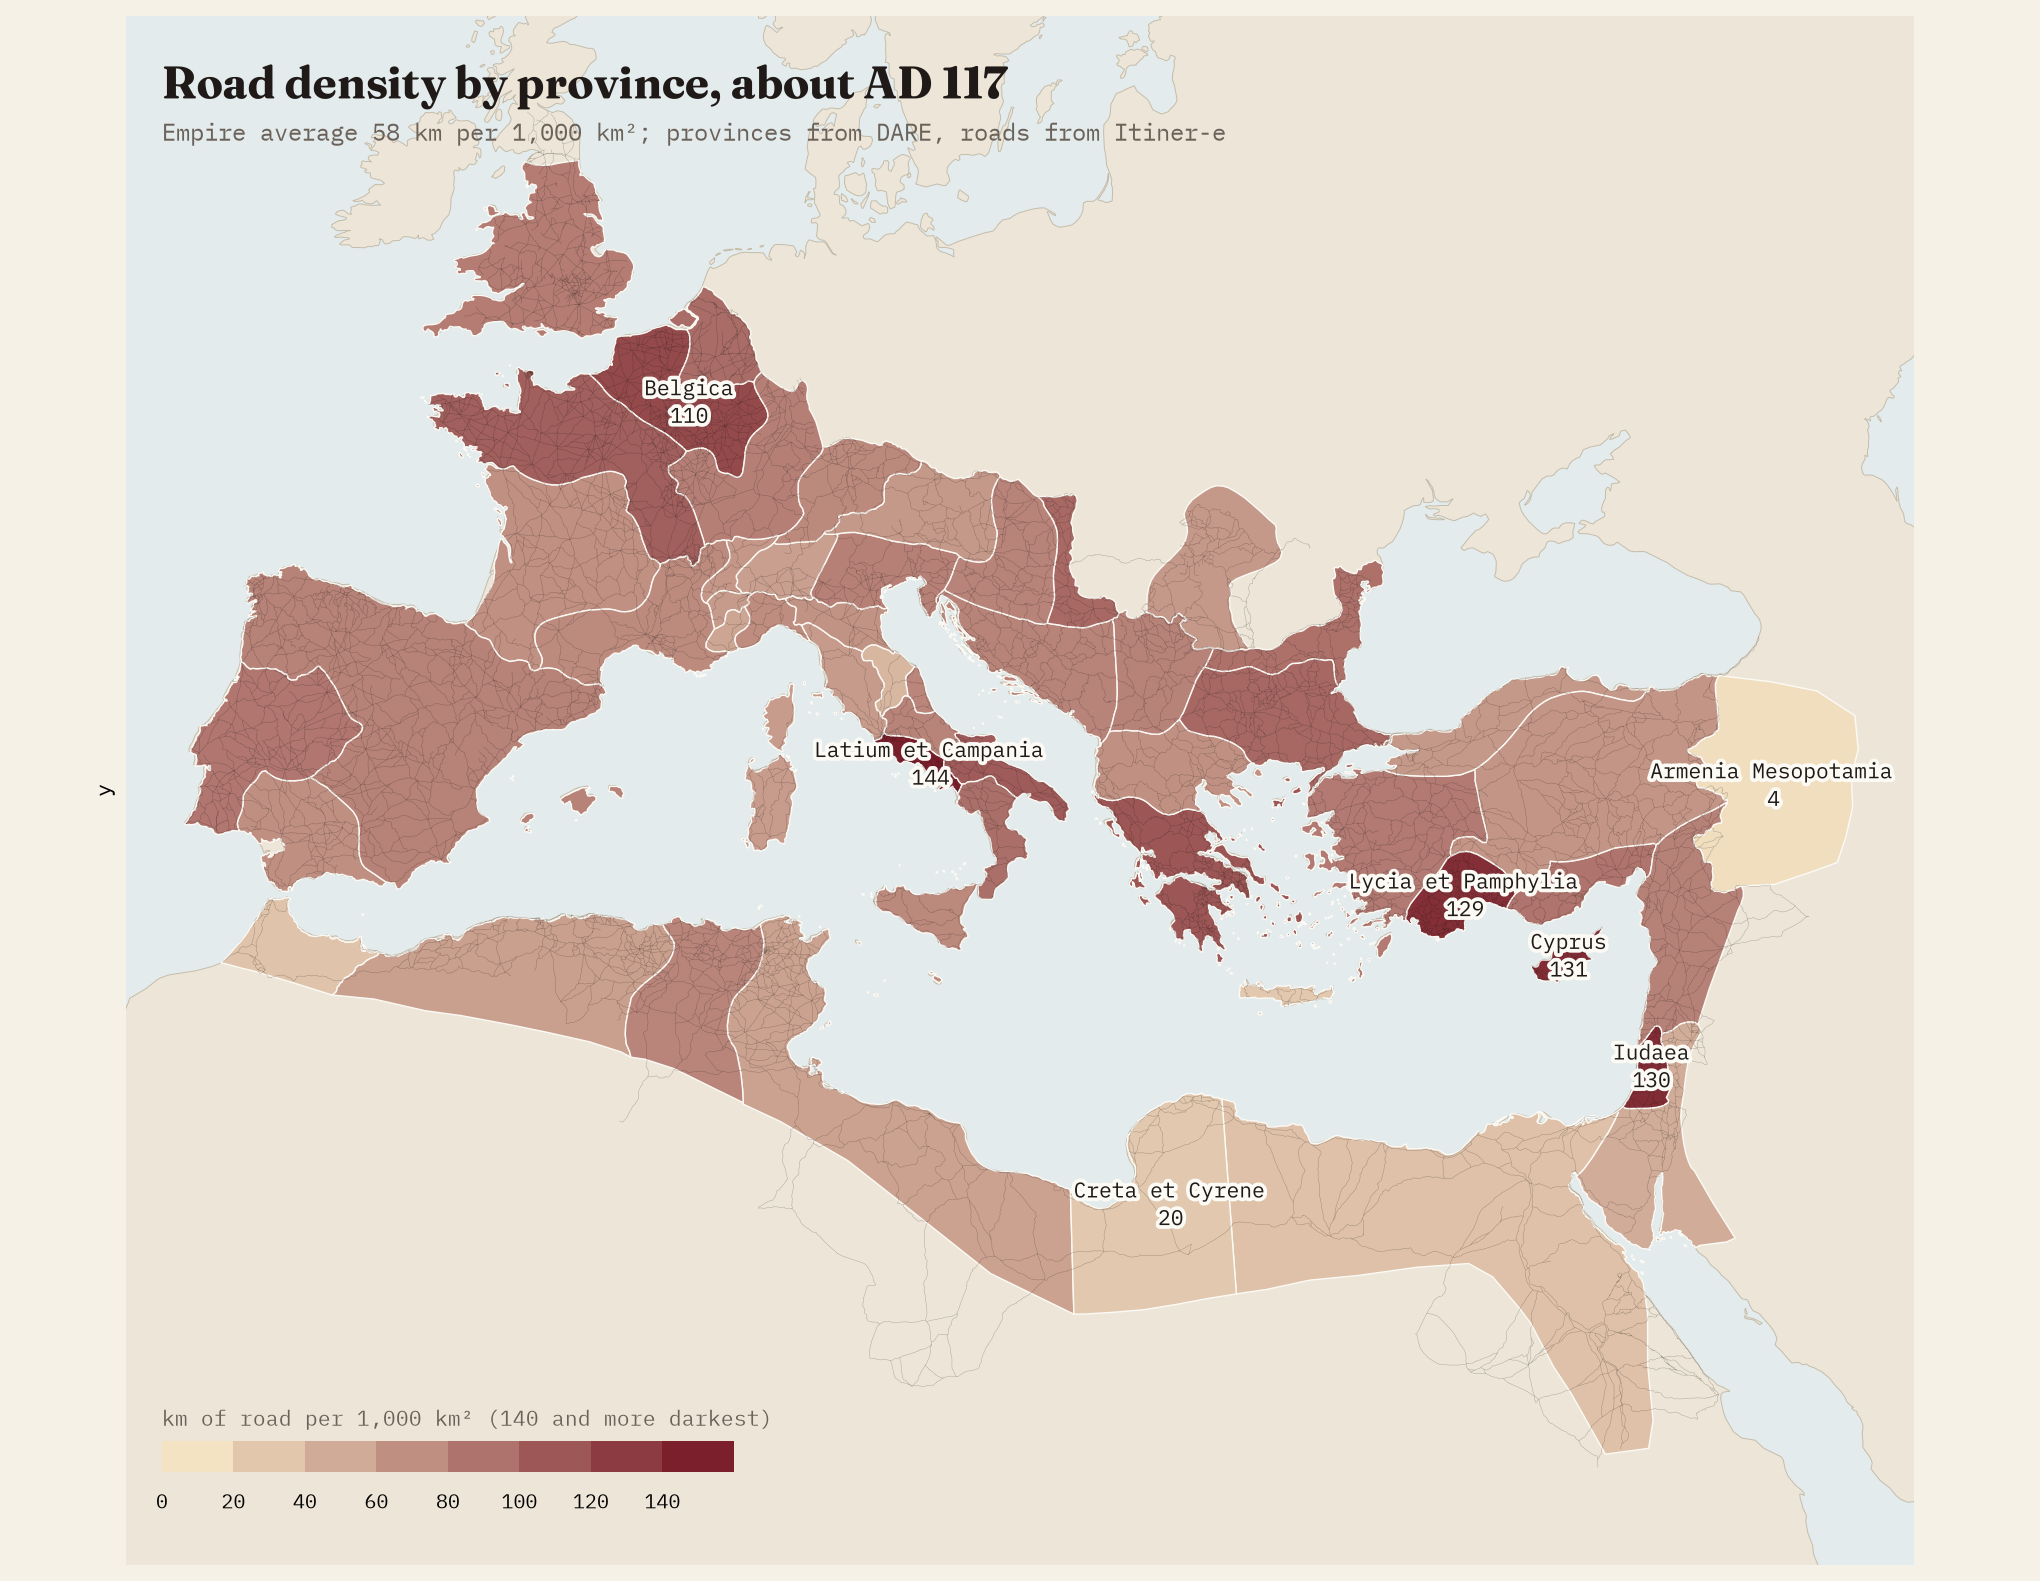
\includegraphics[width=\textwidth]{fig_provinces.png}\caption{Road density by province, about AD 117 (provinces from DARE).}\label{fig:prov}\end{figure}

\begin{table}[tbp]\centering\small\caption{Road density by province, about AD 117: the twelve densest and the five least dense.}\label{tab:prov}\begin{tabular}{lrrrr}\toprule Province & Road km & Land km\textsuperscript{2} & km per 1,000 km\textsuperscript{2} & Certain\\\midrule
Italia, regio I (Latium et Campania) & 1,972 & 13,649 & 144.5 & 8\%\\
Cyprus & 1,274 & 9,741 & 130.8 & 9\%\\
Iudaea & 2,272 & 17,430 & 130.4 & 39\%\\
Lycia et Pamphylia & 5,006 & 38,907 & 128.7 & 5\%\\
Belgica & 9,961 & 90,367 & 110.2 & 3\%\\
Achaia & 8,045 & 79,743 & 100.9 & 4\%\\
Italia, regio II (Apulia et Calabria) & 2,604 & 26,855 & 97.0 & 0\%\\
Lugdunensis & 15,154 & 160,625 & 94.3 & 0\%\\
Thracia & 9,517 & 108,363 & 87.8 & 1\%\\
Pannonia Inferior & 2,501 & 28,667 & 87.2 & 0\%\\
Germania Inferior & 3,709 & 43,598 & 85.1 & 13\%\\
Italia, regio III (Lucania et Bruttii) & 2,320 & 27,949 & 83.0 & 0\%\\
\multicolumn{5}{c}{\dots}\\
Italia, regio VI (Umbria) & 422 & 13,397 & 31.5 & 0\%\\
Aegyptus & 12,721 & 520,437 & 24.4 & 2\%\\
Mauretania Tingitana & 1,166 & 51,497 & 22.6 & 0\%\\
Creta et Cyrene & 3,969 & 202,513 & 19.6 & 0\%\\
Armenia Mesopotamia & 771 & 200,792 & 3.8 & 10\%\\
\bottomrule\end{tabular}\end{table}

\section{Discussion}
The travel-time model is deliberately simple: it asks what the roads alone could do. Its most striking results, Alexandria at 180 days and Carthage at 210, are less statements about Roman travel than about the role of the sea, which no roads-only model can capture. ORBIS \citep{orbis,scheidel2014} models sea, river and road travel together, with seasons and many kinds of traveller, on a coarser road network, and its results show how much faster sea routes usually were for long journeys. The two approaches are complementary: Itiner-e gives a far more detailed picture of how the land was tied together, and a model that combines its roads with sea routes is an obvious next step.

The certainty grades are the dataset's most valuable feature. They show that a map of Roman roads is overwhelmingly a map of reasoned reconstruction: the lines are placed with care, but few have been traced on the ground to within a couple of hundred metres. For travel times this matters little, as errors of a few hundred metres hardly change journeys of weeks. For questions about where roads ran, or which settlements they served, it matters a great deal.

\section{Limitations}
Most of the network is conjectured and only a fifth is dated, so the map is a composite of roads that existed at some point between about 300 BCE and 300 CE, not the network at any one moment. Coverage reflects the uneven history of research. The travel model uses three fixed speeds, an inferred slope penalty that the field description does not define, one day per sea crossing, and no rests, seasons, rivers or sea routes; its times are modelled, not recorded. The province outlines are approximate and of one date. Junction names are inferred and may sometimes be imprecise. The straight-run measure depends on the tolerance and on how each road was digitised.

\section*{Data availability}
Derived data (road sections with travel times, junctions, province densities, straight runs, named roads and the full results) and all code are at \url{https://github.com/Tristan-Hotham/roman-roads} and archived with this paper. Itiner-e is licensed CC BY 4.0, and the derived data, figures and text are shared under the same licence; the code is MIT licensed.

\section*{AI statement}
I wrote the text, with drafting and editing assistance from Claude (Anthropic), which also helped prepare the analysis code. I reviewed and checked all text and results.

\begin{thebibliography}{99}
\bibitem[{\AA}hlfeldt(2026)]{dare} {\AA}hlfeldt, J. (2026) Digital Atlas of the Roman Empire (DARE). Vector data via \url{https://github.com/klokantech/roman-empire}.
\bibitem[de Soto et al.(2025a)]{itinere} de Soto, P., Pa\v{z}out, A., Brughmans, T., Vahlstrup, P. et al. (2025) A high-resolution dataset of roads of the Roman Empire: Itiner-e static version 2024. Zenodo, version 1.3. \url{https://doi.org/10.5281/zenodo.17122148}. CC BY 4.0.
\bibitem[de Soto et al.(2025b)]{desoto2025} de Soto, P., Pa\v{z}out, A., Brughmans, T. et al. (2025) Itiner-e dataset of Roman roads. \emph{Scientific Data}. \url{https://doi.org/10.1038/s41597-025-06140-z}
\bibitem[Dijkstra(1959)]{dijkstra1959} Dijkstra, E.W. (1959) A note on two problems in connexion with graphs. \emph{Numerische Mathematik} 1, 269-271.
\bibitem[Douglas and Peucker(1973)]{douglas1973} Douglas, D.H. and Peucker, T.K. (1973) Algorithms for the reduction of the number of points required to represent a digitized line or its caricature. \emph{Cartographica} 10(2), 112-122.
\bibitem[Natural Earth(2026)]{naturalearth} Natural Earth (2026) 1:10m and 1:50m cultural and physical vectors. Public domain. \url{https://www.naturalearthdata.com/}
\bibitem[Scheidel(2014)]{scheidel2014} Scheidel, W. (2014) The shape of the Roman world: modelling imperial connectivity. \emph{Journal of Roman Archaeology} 27, 7-32.
\bibitem[Scheidel and Meeks(2012)]{orbis} Scheidel, W. and Meeks, E. (2012) ORBIS: The Stanford Geospatial Network Model of the Roman World. \url{https://orbis.stanford.edu/}
\bibitem[Talbert(2000)]{talbert2000} Talbert, R.J.A. (ed.) (2000) \emph{Barrington Atlas of the Greek and Roman World}. Princeton: Princeton University Press.
\bibitem[Thomson and Richardson(1999)]{thomson1999} Thomson, R.C. and Richardson, D.E. (1999) The `good continuation' principle of perceptual organization applied to the generalization of road networks. \emph{Proceedings of the 19th International Cartographic Conference}, Ottawa.
\bibitem[Tobler(1993)]{tobler1993} Tobler, W. (1993) Three presentations on geographical analysis and modeling. \emph{NCGIA Technical Report} 93-1. Santa Barbara: National Center for Geographic Information and Analysis.
\bibitem[Wikipedia(2026)]{wikiroads} Wikipedia contributors (2026) Roman roads. English Wikipedia, revision 1383149720. CC BY-SA 4.0. \url{https://en.wikipedia.org/wiki/Roman_roads}
\end{thebibliography}
\end{document}
